\documentclass{article}

% if you need to pass options to natbib, use, e.g.:
%     \PassOptionsToPackage{numbers, compress}{natbib}
% before loading neurips_2019

% ready for submission
\usepackage{neurips_2019}


% Throughout
\newcommand{\given}{\,|\,}
\newcommand{\compcond}[1]{\big(#1\given-\big)}
\newcommand{\tapprox}{\!\approx\!}
\newcommand{\tequiv}{\!\equiv\!}
\newcommand{\teq}{\!=\!}
\newcommand{\tp}{\!+\!}
\newcommand{\tm}{\!-\!}
\newcommand{\tsim}{\!\sim\!}
\newcommand{\ttimes}{\!\times\!}
\newcommand{\tin}{\!\in\!}

\newcommand{\Eq}[1]{\mathbb{E}_Q\left[#1\right]}
\newcommand{\Vq}[1]{\mathbb{V}_Q\left[#1\right]}
\newcommand{\Gq}[1]{\mathbb{G}_Q\left[#1\right]}
\newcommand{\E}[1]{\mathbb{E}\left[#1\right]}
\newcommand{\V}[1]{\mathbb{V}\left[#1\right]}
\newcommand{\G}[1]{\mathbb{G}\left[#1\right]}
\newcommand{\Gqnot}[2]{\mathbb{G}_{Q_{\backslash #1}}\left[#2\right]}
\newcommand{\Eqnot}[2]{\mathbb{E}_{Q_{\backslash #1}}\left[#2\right]}

% Commands for sampling
\newcommand{\Pois}[1]{\textrm{Pois}\left( #1 \right)}
\newcommand{\Bess}[1]{\textrm{Bessel}\left( #1 \right)}
\newcommand{\Binom}[1]{\textrm{Binom}\left( #1 \right)}
\newcommand{\Gam}[1]{\textrm{Gam}\left( #1 \right)}
\newcommand{\Multi}[1]{\textrm{Multinom}\left( #1 \right)}
\newcommand{\Dirac}[1]{\mathbb{1}\left[ #1 \right]}

% APF
\newcommand{\Yten}{\boldsymbol{Y}}
\newcommand{\osub}{\textrm{i}}
\newcommand{\osubs}{\textbf{\osub}}
\newcommand{\lsubs}{\boldsymbol{\kappa}}
\newcommand{\wsu}[2]{#1_{\subs #2}}
\newcommand{\wsup}[2]{#1_{\subs}^{(#2)}}


\newcommand{\yd}{y_{\osubs}}
\newcommand{\ydk}{y_{\osubs \lsubs}}
\newcommand{\mud}{\mu_{\osubs}}
\newcommand{\mudk}{\mu_{\osubs \lsubs}}
\newcommand{\kappas}{\boldsymbol{\kappa} \in \mathcal{K}}
\newcommand{\sumkappa}{\sum_{\kappas}}


\newcommand{\mask}{b}
\newcommand{\maskten}{\boldsymbol{B}}
\newcommand{\maskd}{\mask_{\osubs}}

\newcommand{\ija}{i {\xrightarrow{a}} j}
\newcommand{\yija}{y_{\ija}}
\newcommand{\maskija}{\mask_{\ija}}

% FROM PrGDS
\newcommand{\ydt}{y^{\mathsmaller{(t)}}_{\osubs}}
\newcommand{\rhot}{\rho^{\mathsmaller{(t)}}}
\newcommand{\thetakt}{\theta_{k}^{\mathsmaller{(t)}}}
\newcommand{\thetakttm}{\theta_{k_2}^{\mathsmaller{(t\!-\!1)}}}
\newcommand{\phikv}{\phi_{kv}}
\newcommand{\epstheta}{\epsilon_0^{\mathsmaller{(\theta)}}}
\newcommand{\epslambda}{\epsilon_0^{\mathsmaller{(\lambda)}}}


\newcommand{\mkt}{m^{\mathsmaller{(t)}}_{k}}
\newcommand{\ykt}{y^{\mathsmaller{(t)}}_{k}}
\newcommand{\yvt}{y^{\mathsmaller{(t)}}_{v}}
\newcommand{\yvtk}{y^{\mathsmaller{(t)}}_{vk}}
\newcommand{\yitk}{y^{\mathsmaller{(t)}}_{\mathbf{v}k}}
\newcommand{\yit}{y^{\mathsmaller{(t)}}_{\mathbf{v}}}
\newcommand{\muitk}{\mu^{\mathsmaller{(t)}}_{\mathbf{v}k}}
\newcommand{\pitk}{p^{\mathsmaller{(t)}}_{\mathbf{v}k}}
\newcommand{\textr}{\textrm{r}}
\newcommand{\thetalam}{\sum_{k_2=1}^K \lambda_{kk_2} \theta_{k_2}^{(t{-}1)}}
\newcommand{\thetapi}{\sum_{k_2=1}^K \pi_{kk_2} \theta_{k_2}^{(t{-}1)}}

\newcommand{\omegakt}{\omega_{k}^{\mathsmaller{(t)}}}
\newcommand{\zetakt}{\zeta_{k}^{\mathsmaller{(t)}}}
\newcommand{\zetaktp}{\zeta_{k}^{(t \tp 1)}}
\newcommand{\deltat}{\delta^{\mathsmaller{(t)}}}
\newcommand{\alphakt}{\alpha_{k}^{\mathsmaller{(t)}}}
\newcommand{\betakt}{\beta_{k}^{\mathsmaller{(t)}}}
\newcommand{\thetaktm}{\theta_{k}^{\mathsmaller{(t\!-\!1)}}}
\newcommand{\thetaktp}{\theta_{k}^{\mathsmaller{(t\!+\!1)}}}
\newcommand{\hkt}{h_k^{\mathsmaller{(t)}}}
\newcommand{\hdkt}{h_{\cdot k}^{\mathsmaller{(t)}}}
\newcommand{\hkdt}{h_{k \cdot}^{\mathsmaller{(t)}}}
\newcommand{\hktm}{h_{k}^{\mathsmaller{(t\!-\!1)}}}
\newcommand{\hktp}{h_{k}^{\mathsmaller{(t\!+\!1)}}}
\newcommand{\hdktp}{h_{\cdot k}^{\mathsmaller{(t\!+\!1)}}}
\newcommand{\hkdtp}{h_{k \cdot}^{\mathsmaller{(t\!+\!1)}}}
\newcommand{\hkkt}{h_{kk_2}^{\mathsmaller{(t)}}}
\newcommand{\phimki}{\phi_{ki_m}^{(m)}}
\newcommand{\alphamki}{\alpha_{ki_m}^{(m)}}
\newcommand{\betamki}{\beta_{ki_m}^{(m)}}
\newcommand{\tildethetakt}{\tilde{\boldsymbol{\theta}}_{k}^{\mathsmaller{(t)}}}
\newcommand{\tildethetaktm}{\tilde{\boldsymbol{\theta}}_{k}^{(t\tm1)}}
\newcommand{\cm}{c^{(m)}}
\newcommand{\ez}{\epsilon_0}
\newcommand{\lkt}{l_k^{\mathsmaller{(t)}}}
\newcommand{\hypconf}[1]{{}_1\textrm{F}_1\left( #1 \right)}


% \newcommand{\prodbeta}{\big(\hspace{-0.25em}\prod_{j \in \mathcal{R}_d}\hspace{-0.25em}\beta_{kj}\big)}
% \newcommand{\prodbetanj}{\big(\hspace{-0.25em}\prod_{j' \in \mathcal{R}_d}\hspace{-0.25em}\beta_{kj'}\big)}
% \newcommand{\lnphi}{\ln(1+\phi_{kv}\,\xi^{-1})}
% \newcommand{\omegarate}{\omega^{(\tau_d)}_{s_d \xrightarrow{k} \mathcal{R}_d}}

% to compile a preprint version, e.g., for submission to arXiv, add add the
% [preprint] option:
    % \usepackage[preprint]{neurips_2019}

% to compile a camera-ready version, add the [final] option, e.g.:
     % \usepackage[final]{neurips_2019}

% to avoid loading the natbib package, add option nonatbib:
%     \usepackage[nonatbib]{neurips_2019}

\PassOptionsToPackage{numbers, compress}{natbib}
\usepackage[utf8]{inputenc} % allow utf-8 input
\usepackage[T1]{fontenc}    % use 8-bit T1 fonts
\usepackage{hyperref}       % hyperlinks
\usepackage{url}            % simple URL typesetting
\usepackage{booktabs}       % professional-quality tables
\usepackage{amsfonts}       % blackboard math symbols
\usepackage{nicefrac}       % compact symbols for 1/2, etc.
\usepackage{microtype}      % microtypography
\usepackage{amsmath}
\usepackage{amssymb} 
\usepackage[capitalise]{cleveref}
\usepackage{graphicx,subfigure}
\usepackage{relsize}
\hypersetup{colorlinks,breaklinks,
            allcolors=[rgb]{0.25,0.5,1}}


\title{Poisson-Randomized Gamma Dynamical Systems}

% The \author macro works with any number of authors. There are two commands
% used to separate the names and addresses of multiple authors: \And and \AND.
%
% Using \And between authors leaves it to LaTeX to determine where to break the
% lines. Using \AND forces a line break at that point. So, if LaTeX puts 3 of 4
% authors names on the first line, and the last on the second line, try using
% \AND instead of \And before the third author name.

\author{%
  Aaron Schein \\
  Data Science Institute\\
  Columbia University\\
  % \texttt{hippo@cs.cranberry-lemon.edu} \\
  % examples of more authors
  \And
  Scott Linderman \\
  Data Science Institute\\
  Columbia University\\
  % \texttt{email} \\
  \AND
  Mingyuan Zhou \\
  McCombs School of Business\\
  University of Texas at Austin\\
  % \texttt{email} \\
  \And
  David Blei \\
  Computer Science Department\\
  Columbia University\\
  % \texttt{email} \\
  \And
  Hanna Wallach \\
  Microsoft Research\\
  New York, NY\\
  % \texttt{email} \\
}

\begin{document}

\maketitle

\begin{abstract}
This paper presents the Poisson-randomized gamma dynamical system (PrGDS), a model for sequentially-observed count tensors that encodes a strong inductive bias towards sparsity and burstiness. The PrGDS is based on a fundamentally new motif in Bayesian latent variable modeling: an alternating series of discrete Poisson and continuous Gamma latent states. This motif is widely applicable and analytically tractable, yielding closed-form complete conditionals for all variables by way of the Bessel distribution and a novel distribution that we call the size-biased confluent hypergeometric distribution. We draw connections to closely-related models and compare the PrGDS to them in experiments on real-world count data of text, international events, and neural spike trains. We find that a sparse variant of the PrGDS---which allows continuous latent states to take values of exactly zero---often obtains the lowest smoothing and forecasting perplexity of all models and is uniquely capable of inferring latent structure that is highly localized in time.~\looseness=-1
\end{abstract}

\section{Introduction}


Political scientists often analyze event counts $y^{\mathsmaller{(t)}}_{\mathsmaller{i \xrightarrow{a}j}}$ of the number of times country $i$ took action $a$ towards country $j$ during time step $t$ \cite{schrodt1995event}. Event data exhibit ``complex dependence structures'' \cite{king2001proper} like coalitions of countries and  bursty temporal dynamics. These dependence structures violate the independence assumptions of the traditional hypothesis testing---some political scientists thus warn against using event data to test theories of international relations \cite{green2001dirty,poast2010mis,erikson2014dyadic} while others advocate for using latent variable models to infer unobserved structure as a way to control for it \cite{stewart2014latent}. The latter approach motivates interpretable yet expressive models, capable of capturing a variety of complex latent structures. Event data sets can be represented as a sequence of count tensors $\Yten^{\mathsmaller{(1)}},\dots,\Yten^{\mathsmaller{(T)}}$ each of which contains the $N \ttimes N \ttimes A$ event counts for that time step for every combination of $N$ sender countries, $N$ receivers, and $A$ action types. Recent work on applying tensor decomposition methods to event data sets \cite{hoff2004modeling,hoff2015multilinear,schein2015bayesian,hoff2016equivariant,schein2016bayesian} suggests that such methods infer interpretable coalition structure among countries and topic structure among actions. Like most tensor decomposition methods though, these methods assume that the sequence of tensors is exchangeable and thus fail to fully capture the temporal structure in the data.~\looseness=-1  
% In parallel, work on applying deep recurrent neural networks to event data suggests such methods may be effective at forecasting \cite{trivedi2017know}. There is generally a gap in the literature between flexible models useful for prediction and parsimonious models useful for a range of exploratory and explanatory tasks that arise in scientific practice.

Sequentially observed count tensors are the object of analysis in many scientific disciplines beyond political science. Neuroscientists, for instance, apply tensor decomposition methods to tensors of neuron spike counts to infer interpretable structure that can be explored to suggest new scientific theories about animal behavior and cognition \cite{williams2018unsupervised}. Count data in general  presents unique statistical challenges. Time series of counts tend to be \emph{bursty} \cite{kleinberg2003bursty} while tensors of counts tend to be \emph{sparse} and \emph{high-dimensional} \cite{chi2012tensors,kunihama2013bayesian}. There exists a general lack of models that are tailored to both the challenging properties count time-series and count tensors.~\looseness=-1
% Many core tasks within machine learning research begin with count-valued time series, like community detection in dynamic networks, topic modeling in document streams, and time-sensitive recommendation. Count-valued time series frequently exhibit patterns like asymmetry (i.e., they cannot dip below zero) and ``burstiness'' (i.e., sudden and extreme occurrence) that violate the assumptions of traditional time-series models. 
In recent years, Poisson factorization has emerged as general framework for modeling sparse count matrices~\cite{canny2004gap,Dunson2005bayesianlatent,titsias2008infinite,cemgil2009bayesian,zhou2011beta,gopalan2013efficient} and tensors \cite{ermis2014bayesian,schein2015bayesian}. While tensor decomposition methods generally scale with the size the tensor, many Poisson factorization models na\"ively yield inference algorithms that scale linearly with only the non-zeros in the tensor. This property allows researchers to efficiently explore latent structure in massive tensors, provided they are sparse. However, this property is unique to a subset of Poisson factorization models that only use non-negative prior distributions---to build such models for complex dependence structures like time series, researchers must therefore construct structured priors without relying on the convenience and analytic tractability of the Gaussian distribution.  Hierarchical compositions of non-negative priors---notably, the gamma and Dirichlet---typically introduce non-conjugate dependencies that require innovative posterior innovative schemes.\looseness=-1

\begin{figure*}[t]
\centering
\subfigure[Poisson--gamma dynamical systems~\cite{schein2016poisson}]
{\label{fig:pgds}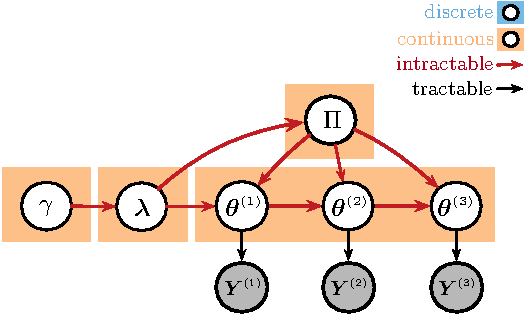
\includegraphics[width=0.49\linewidth]{../../fig/graphical_models/pgds.pdf}}\hfill
% 
\subfigure[Poisson-randomized gamma dynamical systems]
{\label{fig:prgds}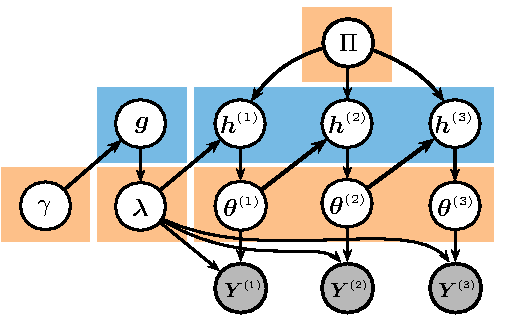
\includegraphics[width=0.49\linewidth]{../../fig/graphical_models/prgds.pdf}}
\caption{\label{fig:comparison} \footnotesize \emph{Left}: The PGDS imposes dependencies directly between the continuous variables that do not yield closed-form conditional distributions. \emph{Right}: The PrGDS (this paper) breaks the intractable dependencies with discrete Poisson variables---doing so yields closed-form conditionals for all variables with any data augmentation.~\looseness=-1}\vspace{-1.5em}
\end{figure*}

This paper seeks to fill a gap in the literature between Poisson factorization models that are \emph{tractable}---i.e., those that yield closed-form complete conditionals---and those that are \emph{expressive}---i.e., capable of capturing a variety of complex dependence structures. To do so, we introduce a fundamentally new modeling motif---an alternating series of discrete Poisson and continuous gamma latent variables---that is analytically convenient, computationally tractable, and widely applicable. We rely on this motif to construct the Poisson-randomized gamma dynamical system (PrGDS), a model for sequentially observed count tensors. Under a specific hyperparameter setting, the continuous latent states of the PrGDS may take values of \emph{exactly} zero thus encoding a strong inductive bias towards sparsity and burstiness. We find that this variant is uniquely capable of inferring latent structure that is highly localized in time. The PrGDS is closely related to the Poisson--gamma dynamical system (PGDS) \cite{schein2016poisson}. We detail the connection between the two models by representing the PrGDS in terms of the \emph{randomized gamma distribution of the first type} (RG1)~\cite{yuan2000bessel,makarov2010exact}. We also discuss how the PGDS is fundamentally limited by the auxiliary variable scheme it requires to perform inference in its non-conjugate structure. By contrast, without any data augmentation, the PrGDS admits closed-form complete conditionals for all latent variables by way of the little-known Bessel distribution~\cite{yuan2000bessel} and a novel univariate discrete distribution that we derive and call the \emph{size-biased confluent hypergeometric (SCH) distribution}. We compare the smoothing and forecasting ability of the PrGDS to the PGDS and two other baselines on a range of real-world count matrices and tensors of text, international events, and neural spike data. In addition to being uniquely capable of inferring highly localized latent structure, we find that the sparse PrGDS variant often obtains the lowest smoothing and forecasting perplexity of all models.~\looseness=-1

% \pagebreak
\section{Poisson-randomized gamma dynamical systems (PrGDS)}
\label{sec:prgds}

\paragraph{Notation.}Consider a data set of of sequentially observed tensors $\boldsymbol{Y}^{\mathsmaller{(1)}},\dots,\boldsymbol{Y}^{\mathsmaller{(T)}}$. An entry $\ydt \!\in\! \{0,1,2,\dots\}$ in the $t^{\textrm{th}}$ tensor is subscripted by a multi-index $\osubs \equiv (\osub_1,\dots,\osub_M)$ which indexes into the $M$ modes of the tensor. As an example, international event counts $y^{\mathsmaller{(t)}}_{\mathsmaller{i \xrightarrow{a} j}}$ collectively form a sequence of 3-mode count tensors where each multi-index corresponds to a unique combination of sender, receiver, and action type---e.g., $\osubs = (i, j, a)$.

\paragraph{Generative process.} The PrGDS is a form of CP decomposition \cite{harshman1970foundations} that models $\yd$ as
\begin{align}
\label{eq:tensor_likelihood}
\ydt &\sim \textrm{Pois}\Big(\rhot \sum_{k = 1}^K \lambda_k \, \thetakt \prod_{m=1}^M \phi^{\mathsmaller{(m)}}_{k \osub_m}\Big).
\end{align}
Here $\thetakt$ represents the strength of the $k^{\textrm{th}}$ latent \emph{component} at time step $t$. Each component describes a particular dependence structure in the data by way of a factor vector $\boldsymbol{\phi}^{\mathsmaller{(m)}}_{k}$ for each mode $m$. For international events data, the first factor vector $\boldsymbol{\phi}^{\mathsmaller{(1)}}_{k} \teq (\phi^{\mathsmaller{(1)}}_{k1},\dots,\phi^{\mathsmaller{(1)}}_{kV})$ would describe the rate at which each of the $V$ countries acts as a sender in the $k^{\textrm{th}}$ component while the second $\boldsymbol{\phi}^{\mathsmaller{(2)}}_{k}$ would describe the rate at which each acts as a receiver. The weights $\lambda_k$ and $\rho^{\mathsmaller{(t)}}$ represent the overall strengths of component $k$ and time step $t$. We call the PrGDS \emph{stationary} if $\rhot \teq \rho$. We assume conjugate gamma and Dirichlet priors over $\rho^{\mathsmaller{(t)}}$ (or $\rho$) and $\boldsymbol{\phi}^{\mathsmaller{(m)}}_{k}$:~\looseness=-1
% there is a set of factors $\phi^{\mathsmaller{(m)}}_{k \osub_m}$ for each mode $m$ that represents the strength of feature $i_{m}$ in component $k$. An analogous generalization can be made of the PGDS. However, as before, the ``augment-and-conquer'' inference is only available if $\lambda_k=\lambda$ and $\sum_{i_m=1}^{L_m} \phi^{\mathsmaller{(m)}}_{k \osub_m} \teq 1$ for all $m$. A secondary contribution of this paper is the generalization of the PGDS to tensor-valued time series which we use in \cref{sec:experiments} as a baseline. We provide the relevant inference equations in the Appendix and will open source our Cython implementation.
\begin{equation}
\rhot \sim \Gam{a_0, b_0} \,\,\,\textrm{ and }\,\,\, \boldsymbol{\phi}^{\mathsmaller{(m)}}_k \sim \textrm{Dir}(a_0,\dots,a_0).
\end{equation}
The PrGDS is characterized by an alternating series of discrete and continuous latent states. The \emph{continuous latent states} $\thetakt$ evolve via intermediate discrete states $\hkt$ from $t=1,\dots,T$ as~\looseness=-1
\begin{equation}
\label{eq:thetaktandhkt}
\thetakt \sim \Gam{\epstheta \tp \hkt,\, \tau} \,\,\textrm{ and }\,\, \hkt \sim \textrm{Pois}\Big(\tau \sum_{k_2 = 1}^K \pi_{kk_2} \,\thetakttm\Big),
\end{equation}
where for $t\teq 0$ we define $\theta^{\mathsmaller{(0)}}_k \teq \lambda_k$ to be the per-component weight that also appears in \cref{eq:tensor_likelihood}. The PrGDS assumes $\thetakt$ is conditionally gamma distributed with \emph{rate} $\tau$ and shape equal to a latent count $\hkt$ plus hyperparameter $\epstheta \geq 0$. We adopt the convention that a gamma random variable is zero, almost surely, if its shape parameter is zero---thus, setting $\epstheta \teq 0$ defines a \emph{sparse variant} of the PrGDS wherein the continuous states are exactly zero $\thetakt \teq 0$ if $\hkt \teq 0$. The \emph{transition weights} $\pi_{kk_2}$ in the Poisson rate of $\hkt$ represent how strongly each component $k_2$ excites component $k$ at the subsequent time step. We view these weights collectively as a $K \!\times\! K$ transition matrix $\Pi$ and impose Dirichlet priors over its columns. We also impose a gamma prior over the \emph{concentration parameter} $\tau$ which is conjugate to both the gamma and Poisson distributions it appears in:~\looseness=-1
\begin{equation}
\tau \sim \Gam{\alpha_0, \alpha_0} \,\,\textrm{ and }\,\,
\boldsymbol{\pi}_k \sim \textrm{Dir}\left(a_0,\dots,a_0\right) \textrm{ such that }\mathsmaller{\sum_{k_1}}^K \pi_{k_1k}=1.
\end{equation}
% \begin{align}
% \mathbb{E}\left[\boldsymbol{\theta}^{\mathsmaller{(t)}} \given \boldsymbol{\theta}^{\mathsmaller{(t \tm 1)}}\right] = \mathbb{E}\left[\mathbb{E}\left[\boldsymbol{\theta}^{\mathsmaller{(t)}} \given \boldsymbol{h}^{\mathsmaller{(t \tm 1)}}\right]\right] = \Pi \, (\boldsymbol{\theta}^{\mathsmaller{(t \tm 1)}} \odot \boldsymbol{\eta}) 
% \end{align}
% When $\epstheta > 0$, this construction corresponds to the \emph{randomized gamma of the first type}~\citep{yuan2000bessel,makarov2010exact} while when $\epstheta=0$ this construction corresponds to the Poisson-randomized gamma distribution~\citep{zhou2016augmentable}.
% Thus, $\tau$ mainly controls the variance of the latent dynamics while only affecting the expectation by a factor of $\epstheta$ (and not at all when $\epstheta \teq 0$). We impose the  prior $\tau \sim \Gam{\alpha_0, \alpha_0}$ which is conjugate to both the Poisson and gamma distributions in which $\tau$ appears.
For the per-component weights $\lambda_k$, we impose a hierarchical prior with a similar flavor to \cref{eq:thetaktandhkt}:~\looseness=-1 
\begin{equation}
\label{eq:lambdakandgk}
\lambda_k \sim \textrm{Gam}\Big(\tfrac{\epslambda}{K} + g_k,\, \beta\Big) \,\,\textrm{ and }\,\,g_k \sim \Pois{\tfrac{\gamma}{K}},
% 
\end{equation}
where $\epslambda$ is a hyperparameter analogous to $\epstheta$. The following gamma priors are then both conjugate:~\looseness=-1
\begin{equation}
\gamma \sim \Gam{a_0,b_0} \,\,\,\textrm{ and }\,\,\, \beta \sim \Gam{\alpha_0, \alpha_0}.
\end{equation}
\paragraph{Properties.}
Both $\epslambda$ and $\gamma$ are divided by the number of components $K$ in \cref{eq:lambdakandgk}---as the number of components grows $K \!\rightarrow\! \infty$, the expected sum of the weights thus remains finite and fixed:~\looseness=-1
\begin{equation}
\sum_{k=1}^\infty \E{\lambda_k} = \sum_{k=1}^\infty \big(\tfrac{\epslambda}{K} + \E{g_k}\big) \beta^{-1} = \sum_{k=1}^\infty \big(\tfrac{\epslambda}{K} + \tfrac{\gamma}{K} \big)\beta^{-1} = \big(\epslambda + \gamma \big)\beta^{-1}.
\end{equation}
Thus, this prior thus encodes an inductive bias towards small values of $\lambda_k$ and may be interpreted as the finite truncation of a novel Bayesian nonparametric process. A small value of $\lambda_k$ shrinks the Poisson rates of both the data $\ydt$ and the first discrete latent state $h^{\mathsmaller{(0)}}_k$---this prior thus encourages the model to only infer components that are both predictive of the data and useful for fitting the latent dynamics.~\looseness=-1


The marginal expectation of the state vector $\boldsymbol{\theta}^{\mathsmaller{(t)}}$ takes the canonical form of linear dynamical systems,~\looseness=-1
\begin{align}
\mathbb{E}\left[\boldsymbol{\theta}^{\mathsmaller{(t)}} \given \boldsymbol{\theta}^{\mathsmaller{(t \tm 1)}}\right] = \mathbb{E}\left[\mathbb{E}\left[\boldsymbol{\theta}^{\mathsmaller{(t)}} \given \boldsymbol{h}^{\mathsmaller{(t \tm 1)}}\right]\right] = \epstheta \tau^{-1} + \Pi \, \boldsymbol{\theta}^{\mathsmaller{(t \tm 1)}},
\end{align}
since by iterated expectation $\E{\thetakt} \teq \big(\epstheta \tp \E{\hkt}\big)\tau^{-1} \teq \big(\epstheta \tp \tau \sum_{k_2 = 1}^K \pi_{kk_2} \,\thetakttm \big) \tau^{-1}$. The \emph{concentration parameter} $\tau$ appears in both the Poisson and gamma distributions in \cref{eq:thetaktandhkt} and thus contributes to the variance of the process while canceling out of the expectation, except for the additive term $\epstheta \tau^{-1}$ which vanishes when $\epstheta \teq 0$.

More generally, we can marginalize out all of the discrete latent states $\hkt$ to obtain a purely continuous dynamical system in terms of the \emph{randomized gamma distribution of the first type} (RG1) \cite{yuan2000bessel,makarov2010exact},~\looseness=-1
\begin{equation}
\
\thetakt \sim \textrm{RG1}\Big(\epstheta,\,\tau\sum_{k_2=1}^K \pi_{kk_2} \thetakttm,\, \tau\Big),
% 
% \,\,\textrm{ such that }\,\, \mathbb{E}\left[\boldsymbol{\theta}^{\mathsmaller{(t)}} \given \boldsymbol{\theta}^{\mathsmaller{(t \tm 1)}}\right] = \tfrac{\epstheta}{\tau} + \Pi \, \boldsymbol{\theta}^{\mathsmaller{(t \tm 1)}}.
\end{equation}
when $\epstheta > 0$ and in terms of a limiting form of the RG1 when $\epstheta \teq 0$. We describe the RG1 in \cref{fig:rg1}.~\looseness=-1

% The PRGDS has five fixed hyperparameters $\epstheta,\epslambda,\alpha_0,a_0,$ and $b_0$. We use $a_0\teq b_0 \teq 0.01$ to define weakly informative gamma and Dirichlet priors and set $\alpha_0 \teq 10$ to define a gamma prior that promotes values close to 1. We consider two cases for $\epstheta,\epslambda \in \{0,1\}$. When these hyperparameters are zero---e.g., $\epslambda \teq 0$---the shape of $\lambda_k$ may be zero, if $g_k\teq0$, in which case $\lambda_k \teq 0$, almost surely.~\looseness=-1

% \pagebreak
\section{Related work}
\label{sec:bg}
\begin{figure}[t]
\centering
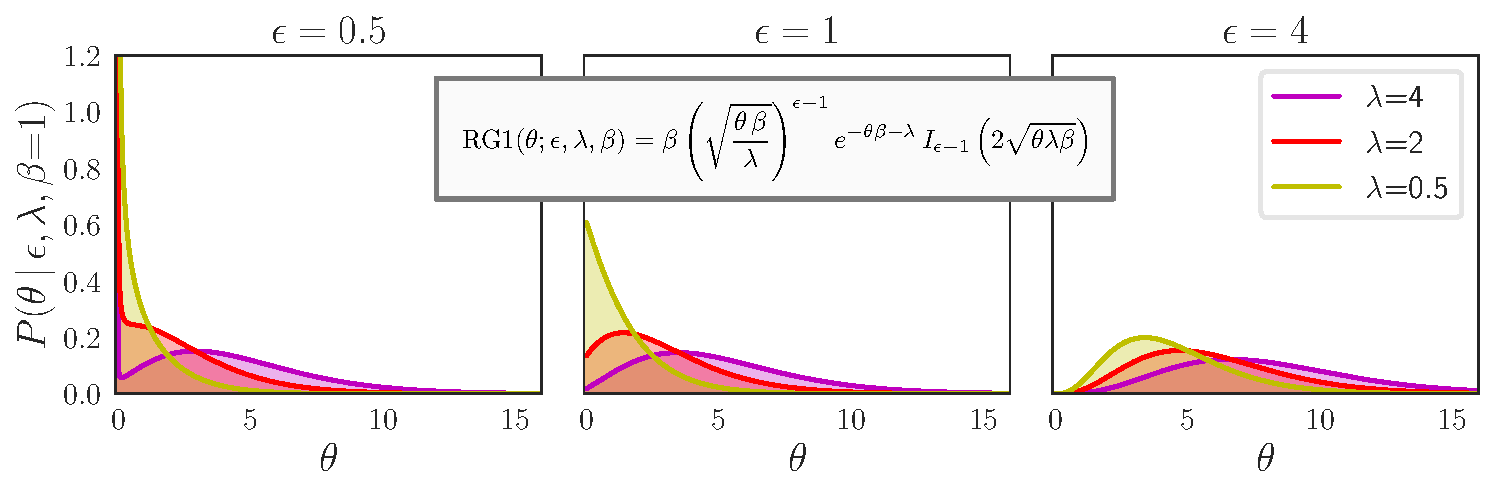
\includegraphics[width=\linewidth]{../../fig/distributions/annotated_rg1.pdf}
\caption{\footnotesize \label{fig:rg1} The randomized gamma distribution of the first type (RG1) \cite{yuan2000bessel,makarov2010exact} has positive support $\theta \!>\!  0$ and is defined by three parameters $\epsilon,\lambda,\beta \!>\! 0$. When $\epsilon < 1$ (\emph{Left}) the RG1 resembles a soft ``spike-and-slab'' while when $\epsilon \geq 1$ (\emph{Middle and Right}) it resembles a more-dispersed form of the gamma distribution. A limiting case of the RG1 when $\epsilon \!\rightarrow\! 0$ is the Poisson-randomized gamma distribution \cite{zhou2016augmentable} which includes zeros in its support $\theta \geq 0$.~\looseness=-1}
\end{figure}
The PrGDS bears a close relationship to the Poisson--gamma dynamical system (PGDS)~\citep{schein2016poisson} wherein~\looseness=-1
\begin{equation}
\label{eq:pgds}
\thetakt \sim \textrm{Gam}\Big(\tau\,\sum_{k_2=1}^K \pi_{kk_2} \thetakttm,\, \tau\Big)\,\,\textrm{ such that }\,\,
% 
\mathbb{E}\left[\boldsymbol{\theta}^{\mathsmaller{(t)}} \given \boldsymbol{\theta}^{\mathsmaller{(t \tm 1)}}\right]= \Pi \, \boldsymbol{\theta}^{\mathsmaller{(t \tm 1)}}.
\end{equation}
The PGDS imposes a direct and non-conjugate dependence between the gamma-distributed states. The complete conditional $P(\thetakt | -)$ is not immediately available in closed form under the PDGS and posterior inference relies on a complicated data augmentation scheme. By contrast, the PrGDS, inserts intermediate Poisson states $\hkt$ that break the intractable dependencies between the gamma states---although the Poisson is not a conjugate prior to the gamma distribution, this construction is still tractable since it yields a closed-form conditional $P(\hkt | -)$, as we'll show in \cref{sec:mcmc}. The PGDS is fundamentally limited by the data augmentation scheme it requires for posterior inference---specifically, this augmentation scheme does not allow any per-component weights $\lambda_k$ to appear in the Poisson rate of $\ydt$ in \cref{eq:tensor_likelihood}. To encourage parsimony, the PGDS instead draws weights $\lambda_k \sim \textrm{Gam}(\tfrac{\gamma}{K}, \beta)$ and uses them to shrink the transition matrix $\Pi$. This introduces more intractable dependencies that necessitate a different augmentation scheme for inference. We provide a graphical comparison of PGDS to PrGDS in \cref{fig:comparison}. In the Appendix, we further detail the limitations of PGDS which also include the restriction that the factors $\boldsymbol{\phi}_k^{\mathsmaller{(m)}}$ and columns $\boldsymbol{\pi}_k$ of the transition matrix are Dirichlet distributed; while we adopt those same assumptions in this paper, the PrGDS is not restricted to them.~\looseness=-1

The PGDS, along with its ``deep'' variants~\cite{gong2017deep,guo2018deep}, generalize gamma process dynamic Poisson factor analysis (GP-DPFA)~\citep{acharya2015nonparametric} which assumes a simple random walk $\thetakt \tsim \Gam{\theta^{\mathsmaller{(t \tm 1)}}_k,\, c^{\mathsmaller{(t)}}}$ that does not express any cross-component excitation (see also a related model~\cite{yang2018dependent}). These models belong to a line of work exploring the application of the ``augment-and-conquer'' data augmentation scheme~\cite{zhou2012augment-and-conquer} to perform inference in hierarchies of gamma variables chained via their shape and linked to Poisson observations---beyond time-series models, this construction can be used to build belief networks~\cite{zhou2015poisson}. An alternative approach is to chain gamma variables via their rate---e.g., $\theta^{\mathsmaller{(t)}} \sim \Gam{a,\,\theta^{\mathsmaller{(t\tm 1)}}}$. This motif has been applied to time-series models~\cite{cemgil2007conjugate,jerfel2016dynamic} as well as deep belief networks~\cite{ranganath2015deep}. This construction is conjugate and tractable. However, since gamma variables are inversely proportional to their rate, such chains insert extra intermediate variables to naturally model time series. Moreover, since the rate contributes quadratically to the variance, gamma rate chains may be highly volatile.~\looseness=-1

Gamma shape and rate chains are just two examples of modeling motifs that are motivated by a non-negativity constraint central to efficient Poisson factorization. In general, Poisson factorization assumes that each observed counts are drawn $\yd \sim \Pois{\mud}$ with latent rate $\mud$ defined to be some function of model parameters. When the rate can be written as a (multi)linear function---i.e., $\mud \teq \sum_{k}\mu_{\osubs k}$---Poisson factorization may be equivalently expressed under its \emph{latent source representation}~\cite{Dunson2005bayesianlatent,cemgil2009bayesian} wherein the observed count is defined $\yd \triangleq \sum_k y_{\osubs k}$ to be the sum of latent sources, each of which is independently Poisson distributed $y_{\osubs k} \sim \Pois{\mu_{\osubs k}}$. Conditioning on the latent sources often induces conditional independences between the latent variables and parameters that facilitates closed-form, efficient, and parallelizable posterior inference---thus, the first step in either MCMC or variational inference is to update the latent sources from their complete conditionals, which is multinomial \cite{steel1953relation}~\looseness=-1,
\begin{equation}
\label{eq:thinning}
\compcond{(y_{\osubs1},\dots,y_{\osubs K})} \sim \Multi{\yd,\, (\mu_{\osubs 1},\dots, \mu_{\osubs K})},
\end{equation}
where we leave implicit the normalization of the non-negative rates $\mu_{\osubs k}$ into a probability vector. When the observed count is zero $\yd \teq 0$, the sources are zero $y_{\osubs k} \teq 0$, almost surely, and no computation is required to update them. Thus, any Poisson factorization model that admits a latent source representation scales linearly with only the non-zero counts in the data. This property is indispensable when modeling count tensors which typically contain exponentially more entries than non-zeros~\cite{bhattacharya2012simplex}. 

Since the latent source representation is only available when the rate $\mud$ is a (multi)linear function of parameters and since the rate must be non-negative, by definition of the Poisson distribution, efficient Poisson factorization is only compatible with non-negative priors over parameters. Modeling time series and other complex dependence structures with efficient Poisson factorization often requires developing novel motifs that notably exclude Gaussian priors which researchers have traditionally relied on for their analytic convenience and tractability. The Poisson LDS, for instance, \cite{macke2011empirical} links the widely-used Gaussian linear dynamical system~\cite{kalman1961new,ghahramani1999learning} to  Poisson observations via an exponential link function $\mud = \exp\left({\sum_k \cdots}\right)$. This is one instance of the generalized linear model (GLM) \cite{nelder1972generalized} approach that relies on a non-linear link function and thus does not yield a latent source representation. Another approach is to use log-normal priors, as in Dynamic Poisson Factorization \cite{charlin2015dynamic}---while this approach satisfies the non-negative constraint, the log-normal is not conjugate to the Poisson and does not closed-form conditionals. We also note a long tradition of autoregressive models for count time series including VAR models~\cite{brandt2012bayesian} and those based on Hawkes processes \cite{blundell2012modelling,simma2012modeling,linderman2014discovering}. This approach avoids the challenge of constructing tractable state-space models from non-negative priors by modeling temporal correlation directly between the count observations. For high-dimensional data, such as sequentially-observed tensors, an autoregressive approach is often untenable. 

% As efficient Poisson factorization is  renewed interest \cite{cemgil2019bayesian}, the 

% The PGDS is thus incompatible with gamma priors over the factors $\phi_{kv}$ which are widely used in practice \cite{cemgil2009bayesian,gopalan2015scalable,schein2015bayesian}. It is also incompatible with per-component weights $\lambda_k$ that are widely used in conjunction with Bayesian nonparametric shrinkage priors for implicit model selection \cite{acharya2015nonparametric,schein2016bayesian}. 

% The concentration parameter $\tau$ in the PGDS is analogous to $\tau$ in the PrGDS in that it affects the variance of the latent dynamics without affecting the expected value. However, unlike in the PrGDS, it is treated as a fixed hyperparameter in the PGDS, since no natural conjugate prior exists when it appears in both the shape and rate of the gamma distribution.



% \section{Background}
% \label{sec:bg}



% The challenge we embrace in this paper is thus to construct expressive and structured priors from only non-negative distributions. A reasonable approach is to use the log-normal as a prior, as in Dynamic Poisson factorization~\cite{charlin2015dynamic}. A more natural approach is to use gamma and Dirichlet priors, which are conjugate to the Poisson distribution and yield analytically closed-form complete conditionals. 

% We take a new approach in this paper. Instead of chaining gamma random variables directly, we introduce alternating chains of conditionally gamma- and Poisson- distributed states. This construction is \emph{semi}-conjugate yet yields closed-form complete conditionals for all states, as we show in \cref{sec:mcmc}.\looseness=-1



% Allocative Poisson matrix factorization \cite{canny2004gap,Dunson2005bayesianlatent,titsias2008infinite,cemgil2009bayesian,zhou2011beta,gopalan2013efficient,paisley2014bayesian}. 

% Non-negative tensor decomposition \citep{cichocki2007non,kolda2009tensor} and probabilistic Poisson tensor decomposition \cite{chi2012tensors}, and Bayesian variants \cite{ermis2014bayesian,schein2015bayesian,schein2016bayesian}.

% See \cite{cemgil2019bayesian} for a review of this area along with connections.

% This family of models is underdeveloped due to the lack of tractable and convenient modeling motifs using only non-negative priors. We introduce a fundamentally novel motif and build a dynamical system with it that uses it to chain together dynamic latent states and uses it to shrink.  


% Models that are not tailored to count data fail to make this distinction and thus tend to waste computation and statistical power on the exponentially-large number of zeros, as if each were as informative as a non-zero observation.


\section{Posterior inference}
\label{sec:mcmc}
The complete conditionals for all latent variables in the PrGDS are immediately available in closed form without any data augmentation. Iteratively re-sampling each variable from its conditional constitutes a Gibbs sampling algorithm. We provide conditionals for the latent variables with non-standard priors here and relegate the rest to the Appendix. The tractability of the PrGDS is tied to the novel modeling motif on which it is based which we first discuss in its general form.~\looseness=-1

\subsection{Poisson--gamma--Poisson recursions}
\label{sec:recursion}
Consider the following model of $m$ involving latent variables $\theta$ and $h$ and fixed $c_1, c_2, c_3, \epstheta >0$:
\begin{equation}
h \sim \Pois{c_1}, \,\,
% 
\theta \sim \Gam{\epstheta \tp h, c_2},\,\,
% 
\textrm{and}\,\, m \sim \Pois{\theta c_3}.
\end{equation}
This model is \emph{semi}-conjugate. The gamma prior of $\theta$ is conjugate to the Poisson and its posterior is
%
\begin{align} 
\label{eq:gamma}
\compcond{\theta} &\sim \Gam{\epstheta \tp h + m,\, c_2 + c_3}.
% 
\intertext{The Poisson prior over $h$ is not conjugate to the gamma--- however the conditional posterior of $h$ is still available in closed form by way of the Bessel distribution \cite{yuan2000bessel} which we define in \cref{fig:bessel}:}
%
\label{eq:bessel}
\compcond{h} &\sim \textrm{Bes}\big(\epstheta \tm 1,\, 2\sqrt{\theta \,c_2\, c_1}\big).
\end{align}
The Bessel distribution can be sampled efficiently \cite{devroye2002simulating}; we will release our Cython implementation. 
Provided that $\epstheta \!>\! 0$, sampling $\theta$ and $h$ iteratively from \cref{eq:gamma,eq:bessel} constitutes a valid Markov chain for posterior inference. When $\epstheta \teq 0$ though, $\theta \teq 0$, almost surely, if $h \teq 0$, and vice versa---thus, this Markov chain has an absorbing condition at $h \teq 0$ and violates detailed balance. In this case, we must therefore sample $h$ with $\theta$ marginalized out---towards that end, we give Theorem 1.~\looseness=-1

\textbf{Theorem 1:} The \emph{incomplete} conditional $P(h\given{-\backslash} \theta)\triangleq \int P(h,\theta\given -)\,\mathbf{d}\theta$ is available in closed form as~\looseness=-1
\begin{align}
\label{eq:sch}
\left(h \given {-\backslash} \theta\right) &\sim
\begin{cases}
\textrm{Pois}\big(\frac{c_1\,c_2}{c_3+c_2}\big) &\textrm{if }m=0\\
\textrm{SCH}\big(m,\, \frac{c_1\,c_2}{c_3+c_2}\big)\, &\textrm{otherwise}
\end{cases}
\end{align}
where SCH is a novel univariate discrete distribution we call the \emph{size-biased confluent hypergeometric distribution}. We define the SCH in \cref{fig:sch} and provide further details about it in the Appendix including a derivation of its mode, how to from sample it, and the proof for Theorem 1.~\looseness=-1

\begin{figure*}[t]
\centering
\subfigure[\footnotesize Bessel distribution~\cite{yuan2000bessel}]
{\label{fig:bessel}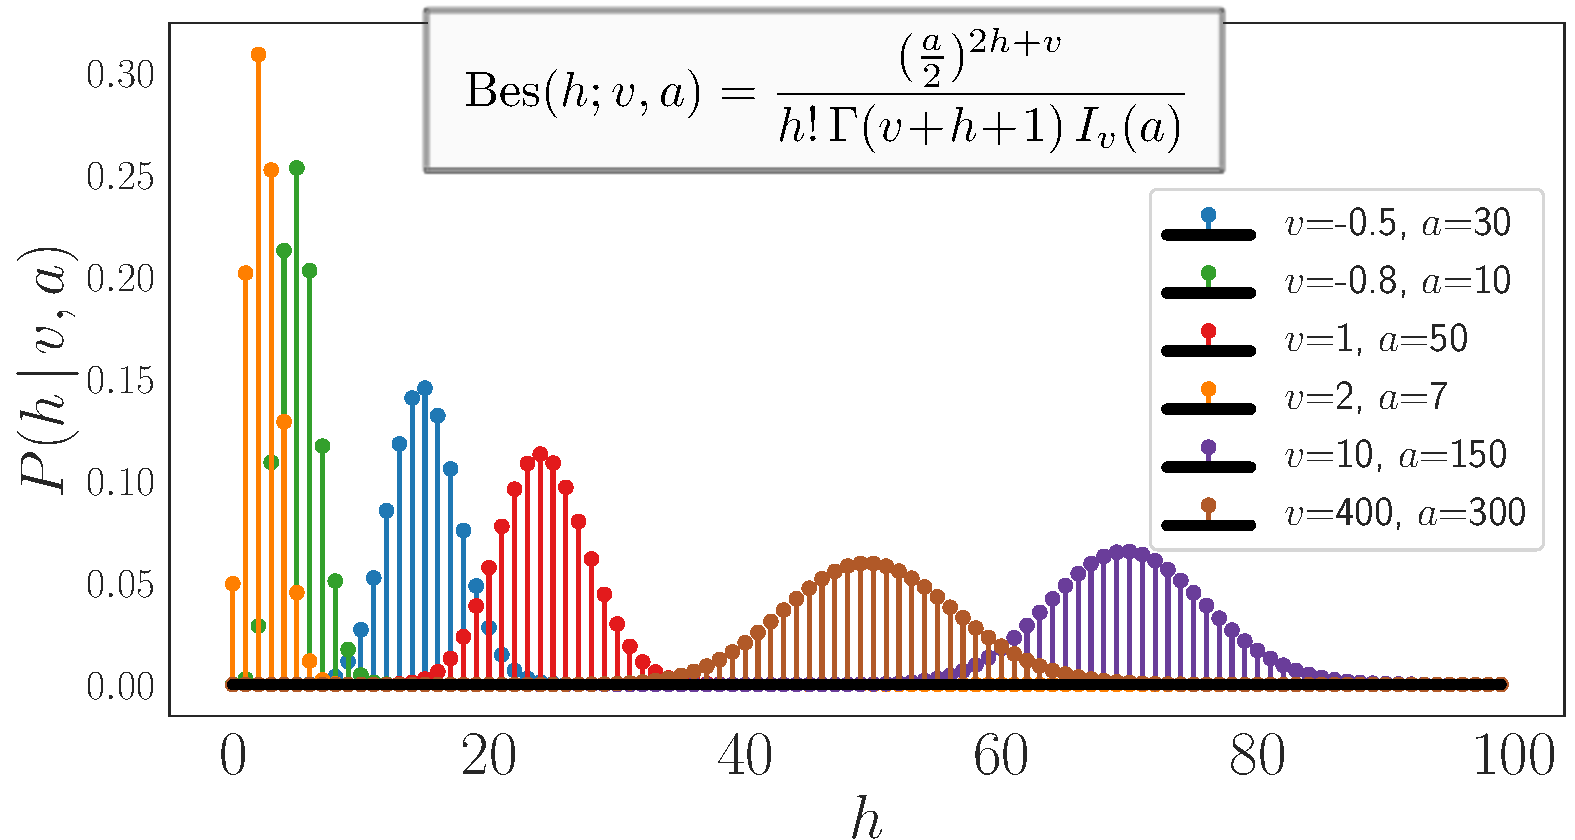
\includegraphics[width=0.49\linewidth]{../../fig/distributions/annotated_bessel.pdf}}\hfill
% 
% \hspace{0.5em}
\subfigure[\footnotesize Size-biased confluent hypergeometric distribution]
{\label{fig:sch}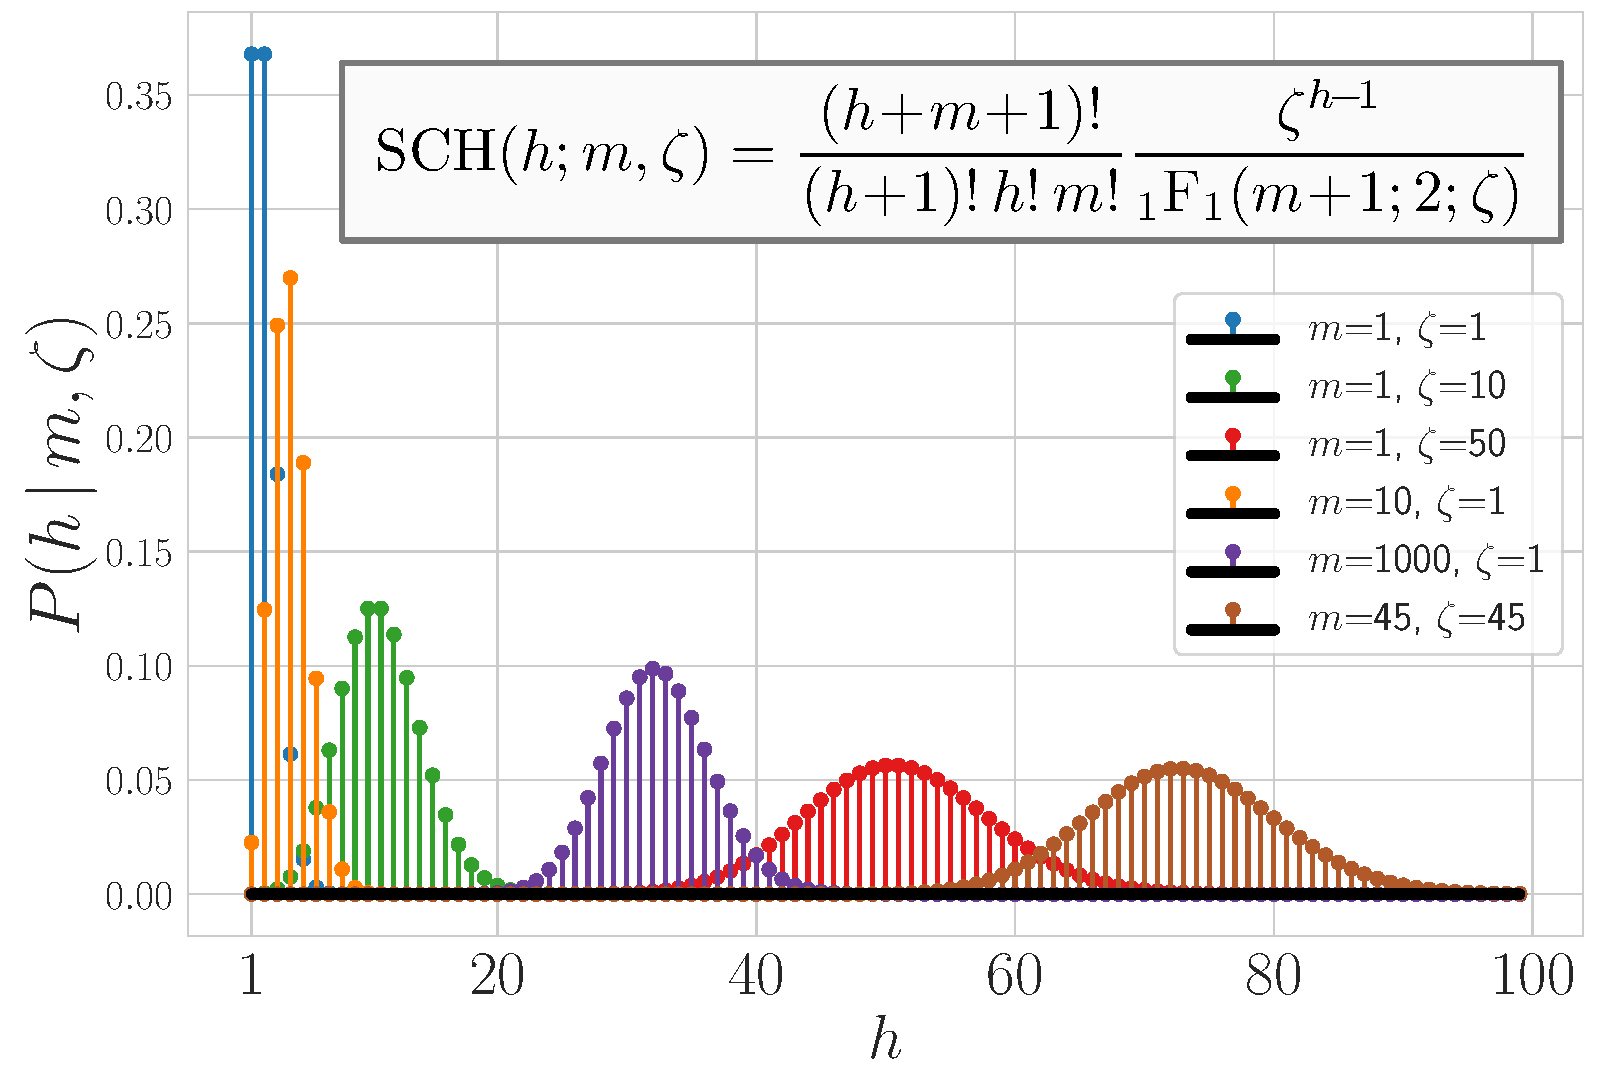
\includegraphics[width=0.49\linewidth]{../../fig/distributions/annotated_sch.pdf}}
\caption{\footnotesize \label{fig:distributions} Two discrete distributions that arise as posteriors in Poisson--gamma--Poisson recursions.~\looseness=-1}
\end{figure*}

\subsection{Closed-form complete conditionals for PrGDS}
The PrGDS yields a latent source representation (see \cref{eq:thinning})---posterior inference thus begins with
\begin{align}
\compcond{(y^{\mathsmaller{(t)}}_{\osubs k})_{k=1}^K} &\sim \Multi{\ydt,\big(\lambda_k \, \thetakt \mathsmaller{\prod}_{m=1}^M \phimki\big)_{k=1}^K},
\intertext{We may similarly represent $\hkt$ under its latent source representation as $\hkt \tequiv \hkdt \teq \sum_{k_2=1}^K \hkkt$ where $\hkkt \tsim \Pois{\tau \, \pi_{kk_2} \thetakttm}$. When useful, we use dot-notation to denote summing over an axis---in this case $\hkdt$ denotes the sum of the $k^{\textrm{th}}$ row of the $K \ttimes K$ matrix of latent counts $\hkkt$. The complete conditional of the $k^{\textrm{th}}$ row of counts, when conditioned on their sum $\hkdt$, is~\looseness=-1}
% 
\compcond{(\hkkt)_{k_2=1}^K} &\sim \Multi{\hkdt,\,(\pi_{kk_2} \thetakttm)_{k_2=1}^K}.
\end{align}
To derive the conditional for $\thetakt$ we aggregate all Poisson variables that depend on it. By Poisson additivity, the column sum $\hdktp \teq \sum_{k_1=1}^K h_{k_1k}^{\mathsmaller{(t \tp 1)}}$ is distributed $\hdktp \tsim \Pois{\thetakt \, \tau\,\pi_{\cdot k}}$ and similarly $y_{\cdot k}^{\mathsmaller{(t)}}$ is distributed $y_{\cdot k}^{\mathsmaller{(t)}} \tsim \textrm{Pois}\big(\thetakt \rhot \lambda_k \prod_{m=1}^M\phi^{\mathsmaller{(m)}}_{k\cdot}\big)$. The count $\mkt \triangleq \hdktp \tp \ykt$ then isolates all dependence on $\thetakt$ and is also Poisson distributed. By gamma--Poisson conjugacy, the conditional of $\thetakt$ is~\looseness=-1
\begin{align}
% \footnote{We provide general equations but note they simplify with Dirichlet priors since $\pi_{\cdot k} \teq 1$ and $\phi^{\mathsmaller{(m)}}_{\cdot k} \teq 1$.~\looseness=-1}
 % 
\compcond{\thetakt} &\sim \textrm{Gam}\big(\epstheta \tp \hkdt + \mkt,\, \tau + \tau\,\pi_{\cdot k}+ \rhot \lambda_k \, \mathsmaller{\prod}_{m=1}^M \phi^{\mathsmaller{(m)}}_{k\cdot }\big).
% 
\intertext{When $\epstheta > 0$, we may apply the identity in \cref{eq:bessel} and sample $\hkdt$ from its complete conditional:}
% 
\compcond{\hkdt} &\sim \textrm{Bessel}\Big(\epstheta \tm 1,\, 2 \sqrt{\thetakt \, \tau^2 \mathsmaller{\sum}_{k_2=1}^K \pi_{kk_2} \thetakttm}\Big).
\end{align}
When $\epstheta \teq0$, we instead apply Theorem 1 to sample $\hkdt$ where $\mkt$ is analogous to $m$ in \cref{eq:sch}:
% 
\begin{align}
\left(\hkdt \given {-\backslash} \thetakt\right) &\sim 
\begin{cases}
\textrm{Pois}(\zeta_{k}^{\mathsmaller{(t)}}) &\textrm{if } \mkt \teq 0 \\ 
% 
\textrm{SCH}(\mkt,\, \zeta_{k}^{\mathsmaller{(t)}}) &\textrm{otherwise}
\end{cases} 
\hspace{1em}\textrm{where }\,\,
\zeta_{k}^{\mathsmaller{(t)}} \triangleq \mathsmaller{\frac{\tau^2 \sum_{k_2=1}^K \pi_{kk_2} \thetakttm}{\tau + \tau\,\pi_{\cdot k} + \rhot \lambda_k \prod_{m=1}^M\phi^{\mathsmaller{(m)}}_{k\cdot }}}.
\end{align}
The conditionals for $\lambda_k$ and $g_k$ follow from applying the same Poisson--gamma--Poisson identities while those for $\gamma$, $\beta$, $\boldsymbol{\phi}^{\mathsmaller{(m)}}_k$, $\boldsymbol{\pi}_{k}$, and $\tau$ all follow from conjugacy. We provide them all in the Appendix.~\looseness=-1
% b

\section{Experiments}
\label{sec:experiments}
In the following series of experiments we compare variants of the PrGDS to each other and existing baselines on their smoothing (i.e., imputing heldout data in the observed time window) and forecasting (i.e., predicting future data). To measure performance, we calculate log perplexity of the non-zero heldout elements $y^{\mathsmaller{(\textrm{test})}}_n \!>\! 0$,~\looseness=-1
% We perform heldout prediction. We calculate perplexity. This is a function of the non-zeros that is related to the posterior predictive. 
\begin{equation}
\label{eq:perplexity}
\log \textrm{Perp}(Y^{\mathsmaller{(\textrm{test})}}) = \frac{1}{N}\sum_{n=1}^N \log \left(\frac{1}{S}\sum_{s=1}^S \textrm{Pois}\left(y^{\mathsmaller{(\textrm{test})}}_n; \mu_n^{(s)}\right) \right)
\end{equation}
where $S$ is the number of MCMC samples and $\mu_n^{\mathsmaller{(s)}}$ is the Poisson rate of the heldout count as defined by the $s^{\textrm{th}}$ sample of model parameters.

\paragraph{Models.} The PrGDS defines a large model family. In these experiments we compare PrGDS variants with $\epstheta \teq 0$ vs.\ 1,  $\epslambda  \teq 0$ vs.\ 1, and Dirichlet versus gamma priors over the non-dynamic factors $\phi^{\mathsmaller{(m)}}_{k \osub_m}$---the cross product of these different choices yields eight PrGDS variants. In the first set of experiments, we follow the experimental design described by Schein et al.~(2016)~\cite{schein2016poisson} on five different dynamic count matrices. We compare the predictive performance of the PrGDS to the performance of the PGDS and GP-DPFA~\cite{acharya2015nonparametric} as baselines. In the next set of experiments, we compare the PrGDS to our tensor generalization of the PGDS on three different dynamic tensors data sets.~\looseness=-1

\subsection{Sequentially observed vectors}
\paragraph{Experimental design.} We replicate the experiments reported by Schein et al.~(2016)
~\cite{schein2016poisson} and apply variants of the PrGDS to the same data sets of dynamic count matrices $Y$ each of size $T \ttimes V$. These include matrices derived from two international event data sets---i.e., GDELT \cite{leetaru2013gdelt} and ICEWS \cite{boscheeicews}---and three text corpora---i.e., NeurIPS papers~\cite{neuripscorpus}, DBLP abstracts~\cite{dblp}, and State of the Union (SOTU) speeches~\cite{sotu}. Details about the experimental design (e.g., number of MCMC samples, random masks, etc.) are given by~\cite{schein2016poisson} which we follow exactly for the PrGDS variants. We obtained from the authors the results for PGDS and GP-DPFA~\cite{acharya2015nonparametric} and used them to compute heldout perplexity.~\looseness=-1


\begin{figure*}[t]
\centering
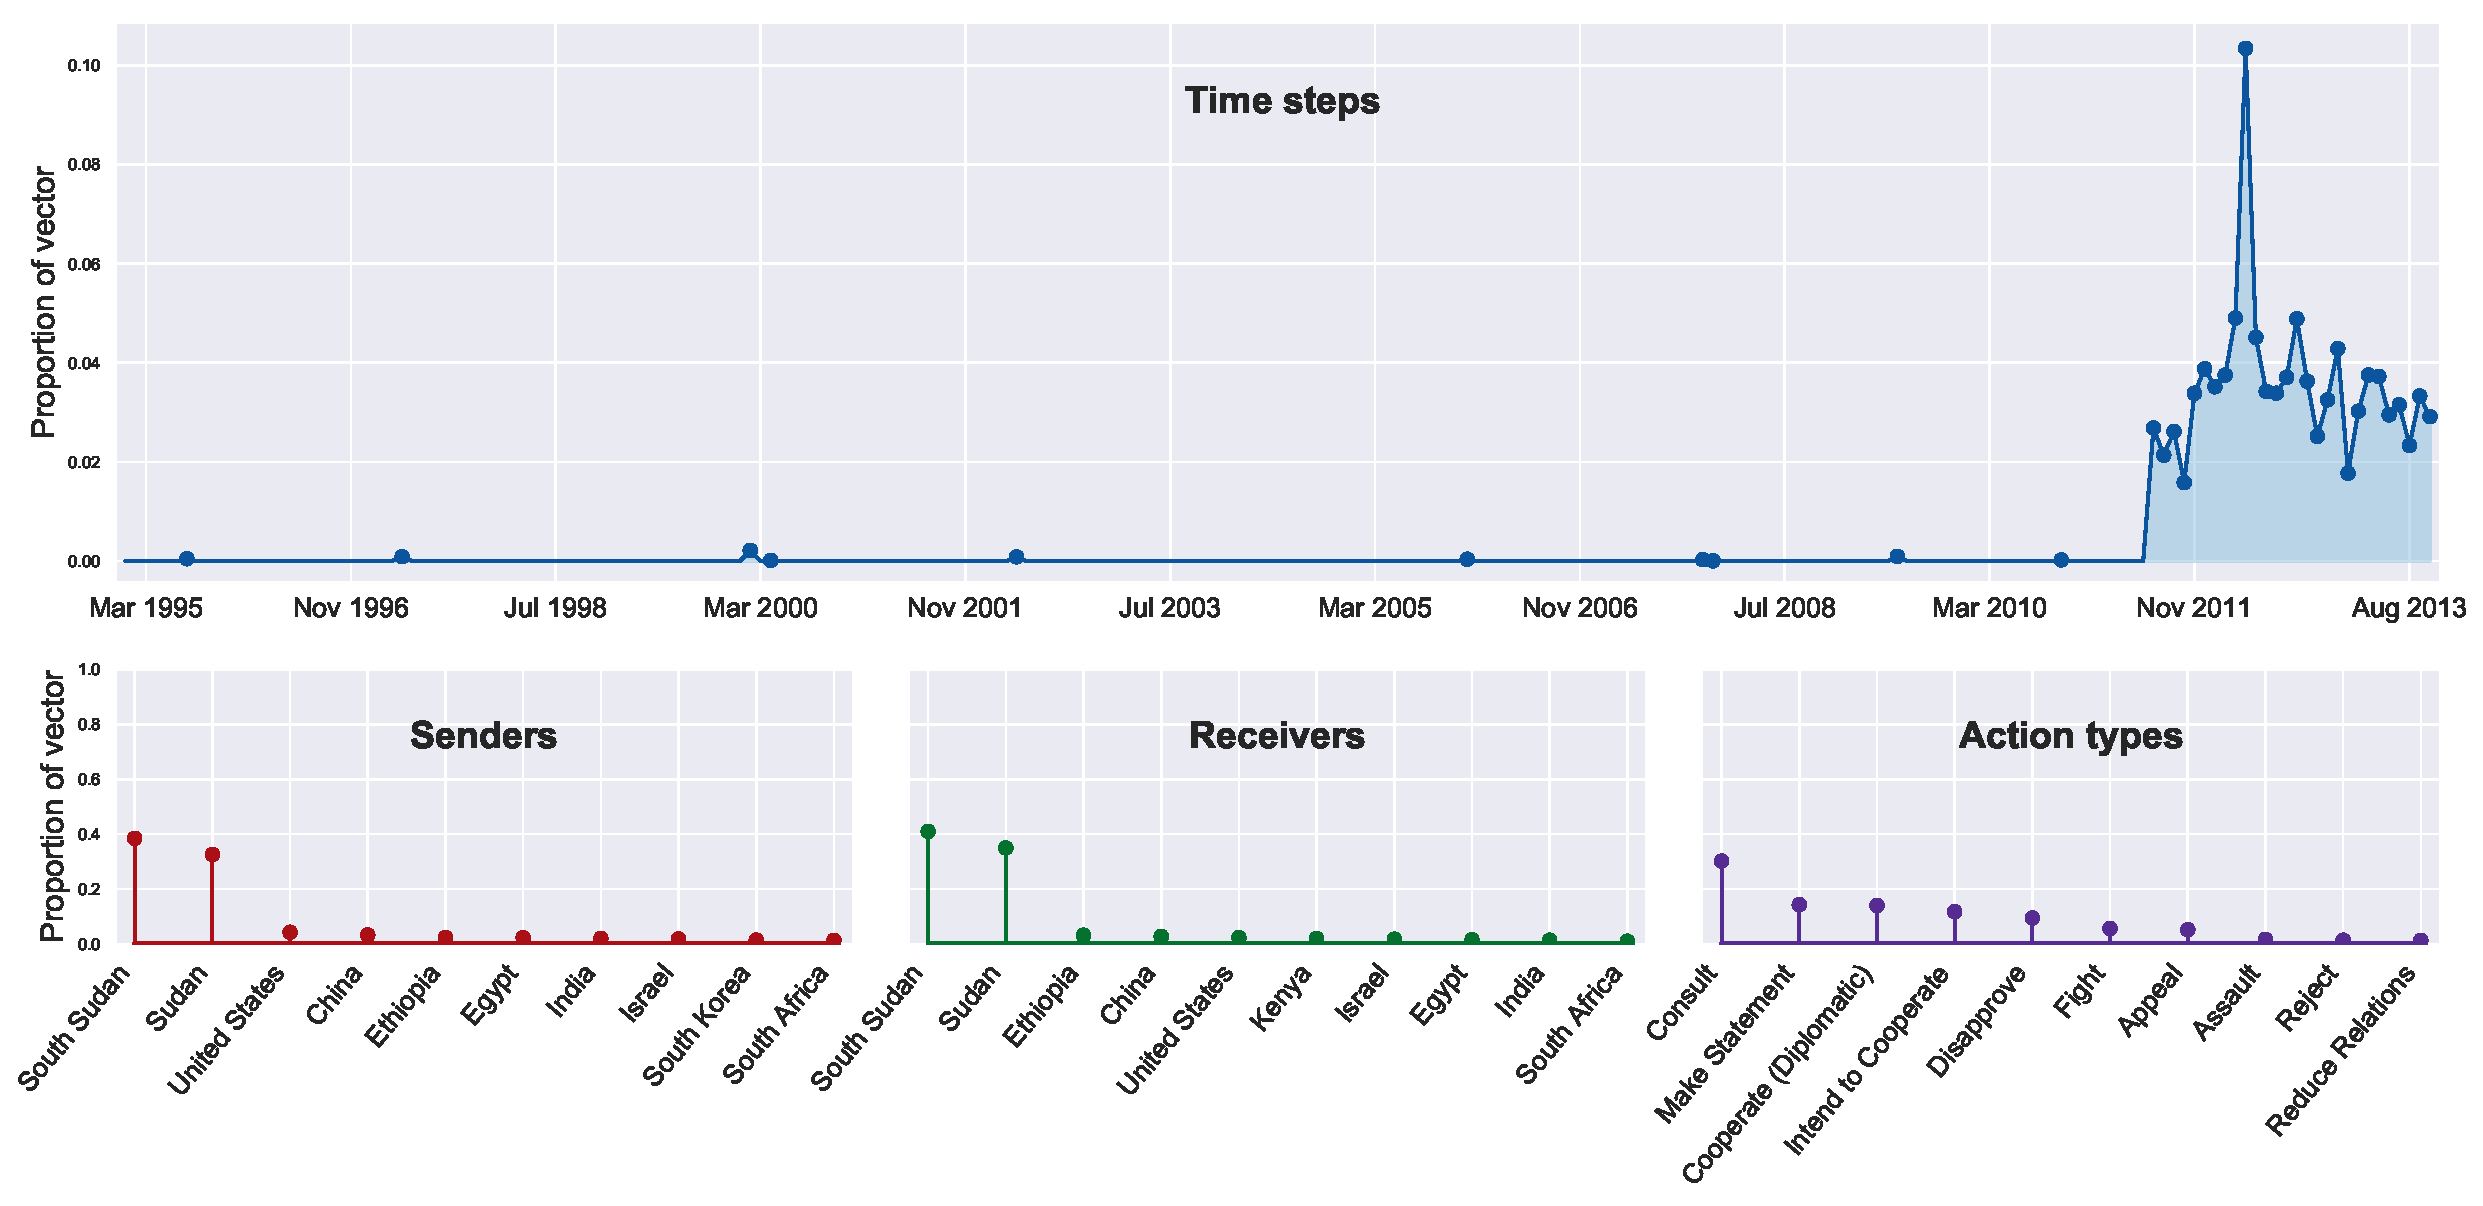
\includegraphics[width=0.9\linewidth]{../../fig/components/icews/zero-ordering/new_plots/eps0-component-0.pdf}
\caption{\footnotesize \label{fig:sudan} A variant of the PrGDS is capable of inferring true sparsity in its continuous latent states. When fit to dynamic tensor data of country--country interactions, this variant inferred the following component. \emph{Top row:} 94\% of the time steps (months) prior to July 2011 exhibit an inferred latent state value of exactly zero $\thetakt \teq 0$. \emph{Bottom left and middle:} This component mainly summarizes events involving South Sudan, a country that did not exist until July 2011. No other variant of the PrGDS found a component dedicated to South Sudan; we speculate that the sparse variant's unique inductive bias allows it surface patterns in the data that are highly localized in time.~\looseness=-1}
\end{figure*}

\paragraph{Results.} See \cref{fig:matrix_results}.
\begin{figure*}[t]
\centering
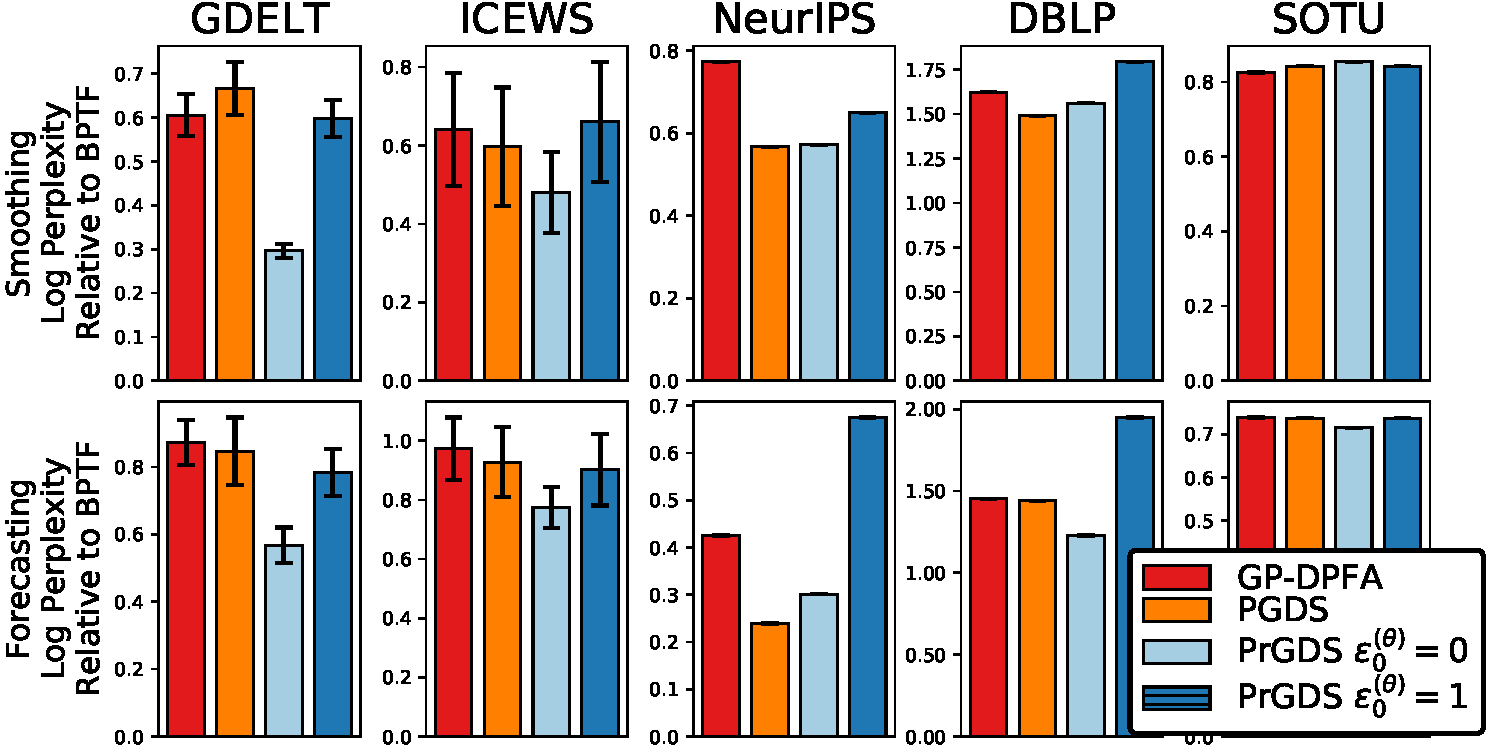
\includegraphics[width=\linewidth]{../../results/matrices/new_matrix_results.pdf}
\caption{\footnotesize \label{fig:matrix_results}Results for the experiments described by Schein~(2016)~\cite{schein2016poisson} for dynamic count matrices. Performance is measured by log perplexity---\emph{lower} is better, see \cref{eq:perplexity}. The top vs.\ bottom rows report smoothing vs.\ forecasting performance for each model, across data sets (columns). In each plot, the baselines are in red (PGDS) and orange (GP-DPFA) while the eight variants of the PrGDS are defined by a combination of color and hatch: i.e., blue vs.\ gamma denotes Dirichlet vs.\ gamma priors, open and closed circles denote $\epstheta \teq 0$ and $\epslambda \teq 0$, respectively, while slanted and straight lines denote $\epstheta \teq 1$ and $\epslambda \teq 1$, respectively. A clear takeaway is the superiority of sparse variant $\epstheta \teq 0$ to the non-sparse one $\epstheta \teq 1$.}
\end{figure*}
\subsection{Sequentially observed tensors}
\paragraph{Experimental design.} For each tensor, we randomly select three pairs of adjacent time steps in the range $[2, T\tm 2]$ to completely hold out---this yields six heldout slices of the tensor $(\Yten^{\mathsmaller(t_1)},\Yten^{\mathsmaller(t_1 \tp 1)}, \Yten^{\mathsmaller(t_2)}, \Yten^{\mathsmaller(t_2 \tp 1)}, \Yten^{\mathsmaller(t_3)}, \Yten^{\mathsmaller(t_3 \tp 1)})$. Additionally, we always hold out the last two slices $(\Yten^{\mathsmaller(T \tm 1)}, \Yten^{\mathsmaller(T)})$. For each data set, we randomly generate two heldout data sets. For each model we run two independent chains of $4,000$ MCMC iterations on each data set and mask combination, saving every $100^{\textrm{th}}$ sample after the first 1,000 to compute log perplexity (as in \cref{eq:perplexity}) on the six intermediate slices (smoothing) and the last two (forecasting).

\paragraph{Data sets.} We created two tensors of international event counts from GDELT~\cite{leetaru2013gdelt} and ICEWS~\cite{boscheeicews}. An entry in one of these tensors contains the count $y_{\mathsmaller{i \xrightarrow{a} j} }^{\mathsmaller{(t)}}$ of how many times country $i$ took action $a$ to country $j$ in time step $t$---each tensor is thus of size $T \ttimes V \ttimes V \ttimes A$ where $V \teq 249$ is the number of countries and $A \teq 20$ is the number of action types. Both tensors treat months as time steps---the GDELT considers the date range 2003--2008 ($T \teq 72$) while the ICEWS tensor considers 1995--2013 ($T \teq 228$).~\looseness=-1

We also consider data of multielectrode recordings of macaque motor cortex from Williams et al.~(2018)~\cite{williams2018unsupervised}. A count in this tensor $y^{\mathsmaller{(t)}}_{ij}$ is number of times neuron $i$ fired in time step $t$ during trial $j$. This tensor is thus size $T \ttimes N \ttimes S$ where $T \teq 162$ is the number of time steps, $N \teq 100$ is the number of recorded neurons, and $S \teq 1,716$ trials.

\paragraph{Results.} See \cref{fig:tensor_results}. We also provide an exploratory analysis of inferred latent structure in \cref{fig:sudan}.

\begin{figure*}[h]
\centering
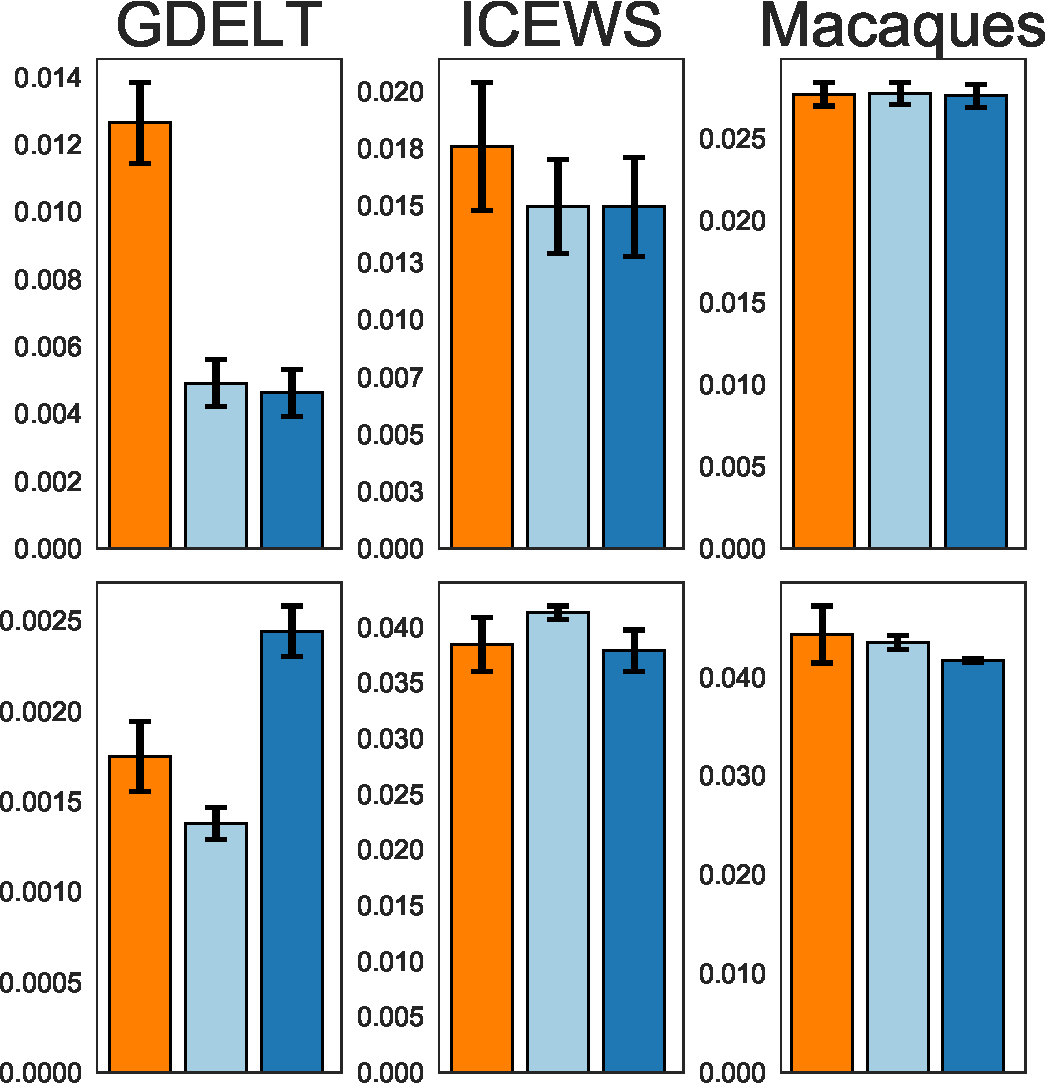
\includegraphics[width=0.75\linewidth]{../../results/tensors/new_tensor_results.pdf}
\caption{\footnotesize\label{fig:tensor_results} Results for the experiments on dynamic count tensors. See the caption of \cref{fig:matrix_results} for description of the legend. Performance is measured by log perplexity where lower is better. Note that the log perplexity scores are negative for the macaque data. One takeaway is that the Dirichlet variants of the PrGDS seem to consistently perform better than the gamma variants.~\looseness=-1}
\end{figure*}





% \section{Discussion}
% \label{sec:conc}

\bibliographystyle{unsrt}
\bibliography{references}

\end{document}